\documentclass[UTF8]{ctexart}

\usepackage{geometry}
\usepackage{graphicx}

\geometry{a4paper, scale=0.9}

\title{低真空获得与测量实验报告}
\author{刘子安 PB20000069}
\date{\today}
\begin{document}
\maketitle

\subsection{低真空}
实验数据:
\begin{table}[!htbp]
	\centering
\begin{tabular}{|c|c|c|c|c|c|c|c|c|c|c|c|c|}
	\hline
	压强 $P(Pa)$ & 20 & 15 & 10 & 9 & 8 & 7 & 6 & 5 & 4.5 & 4 & 3.5 & 3.1 \\
	\hline
	时间 $t(s)$ & 0 & 2.5 & 12 & 17.8 & 25 & 38.8 & 68.1 & 113.5 & 166.6 & 236.4 & 385.8 & 686.3 \\
	\hline
\end{tabular}
\end{table}
\par
从中我们可以得到所组装仪器的极限真空度约为 $P = 3.1 \; Pa$
\par
绘制低真空时的$P-t$图:
\begin{figure}[htb]
	\centering
	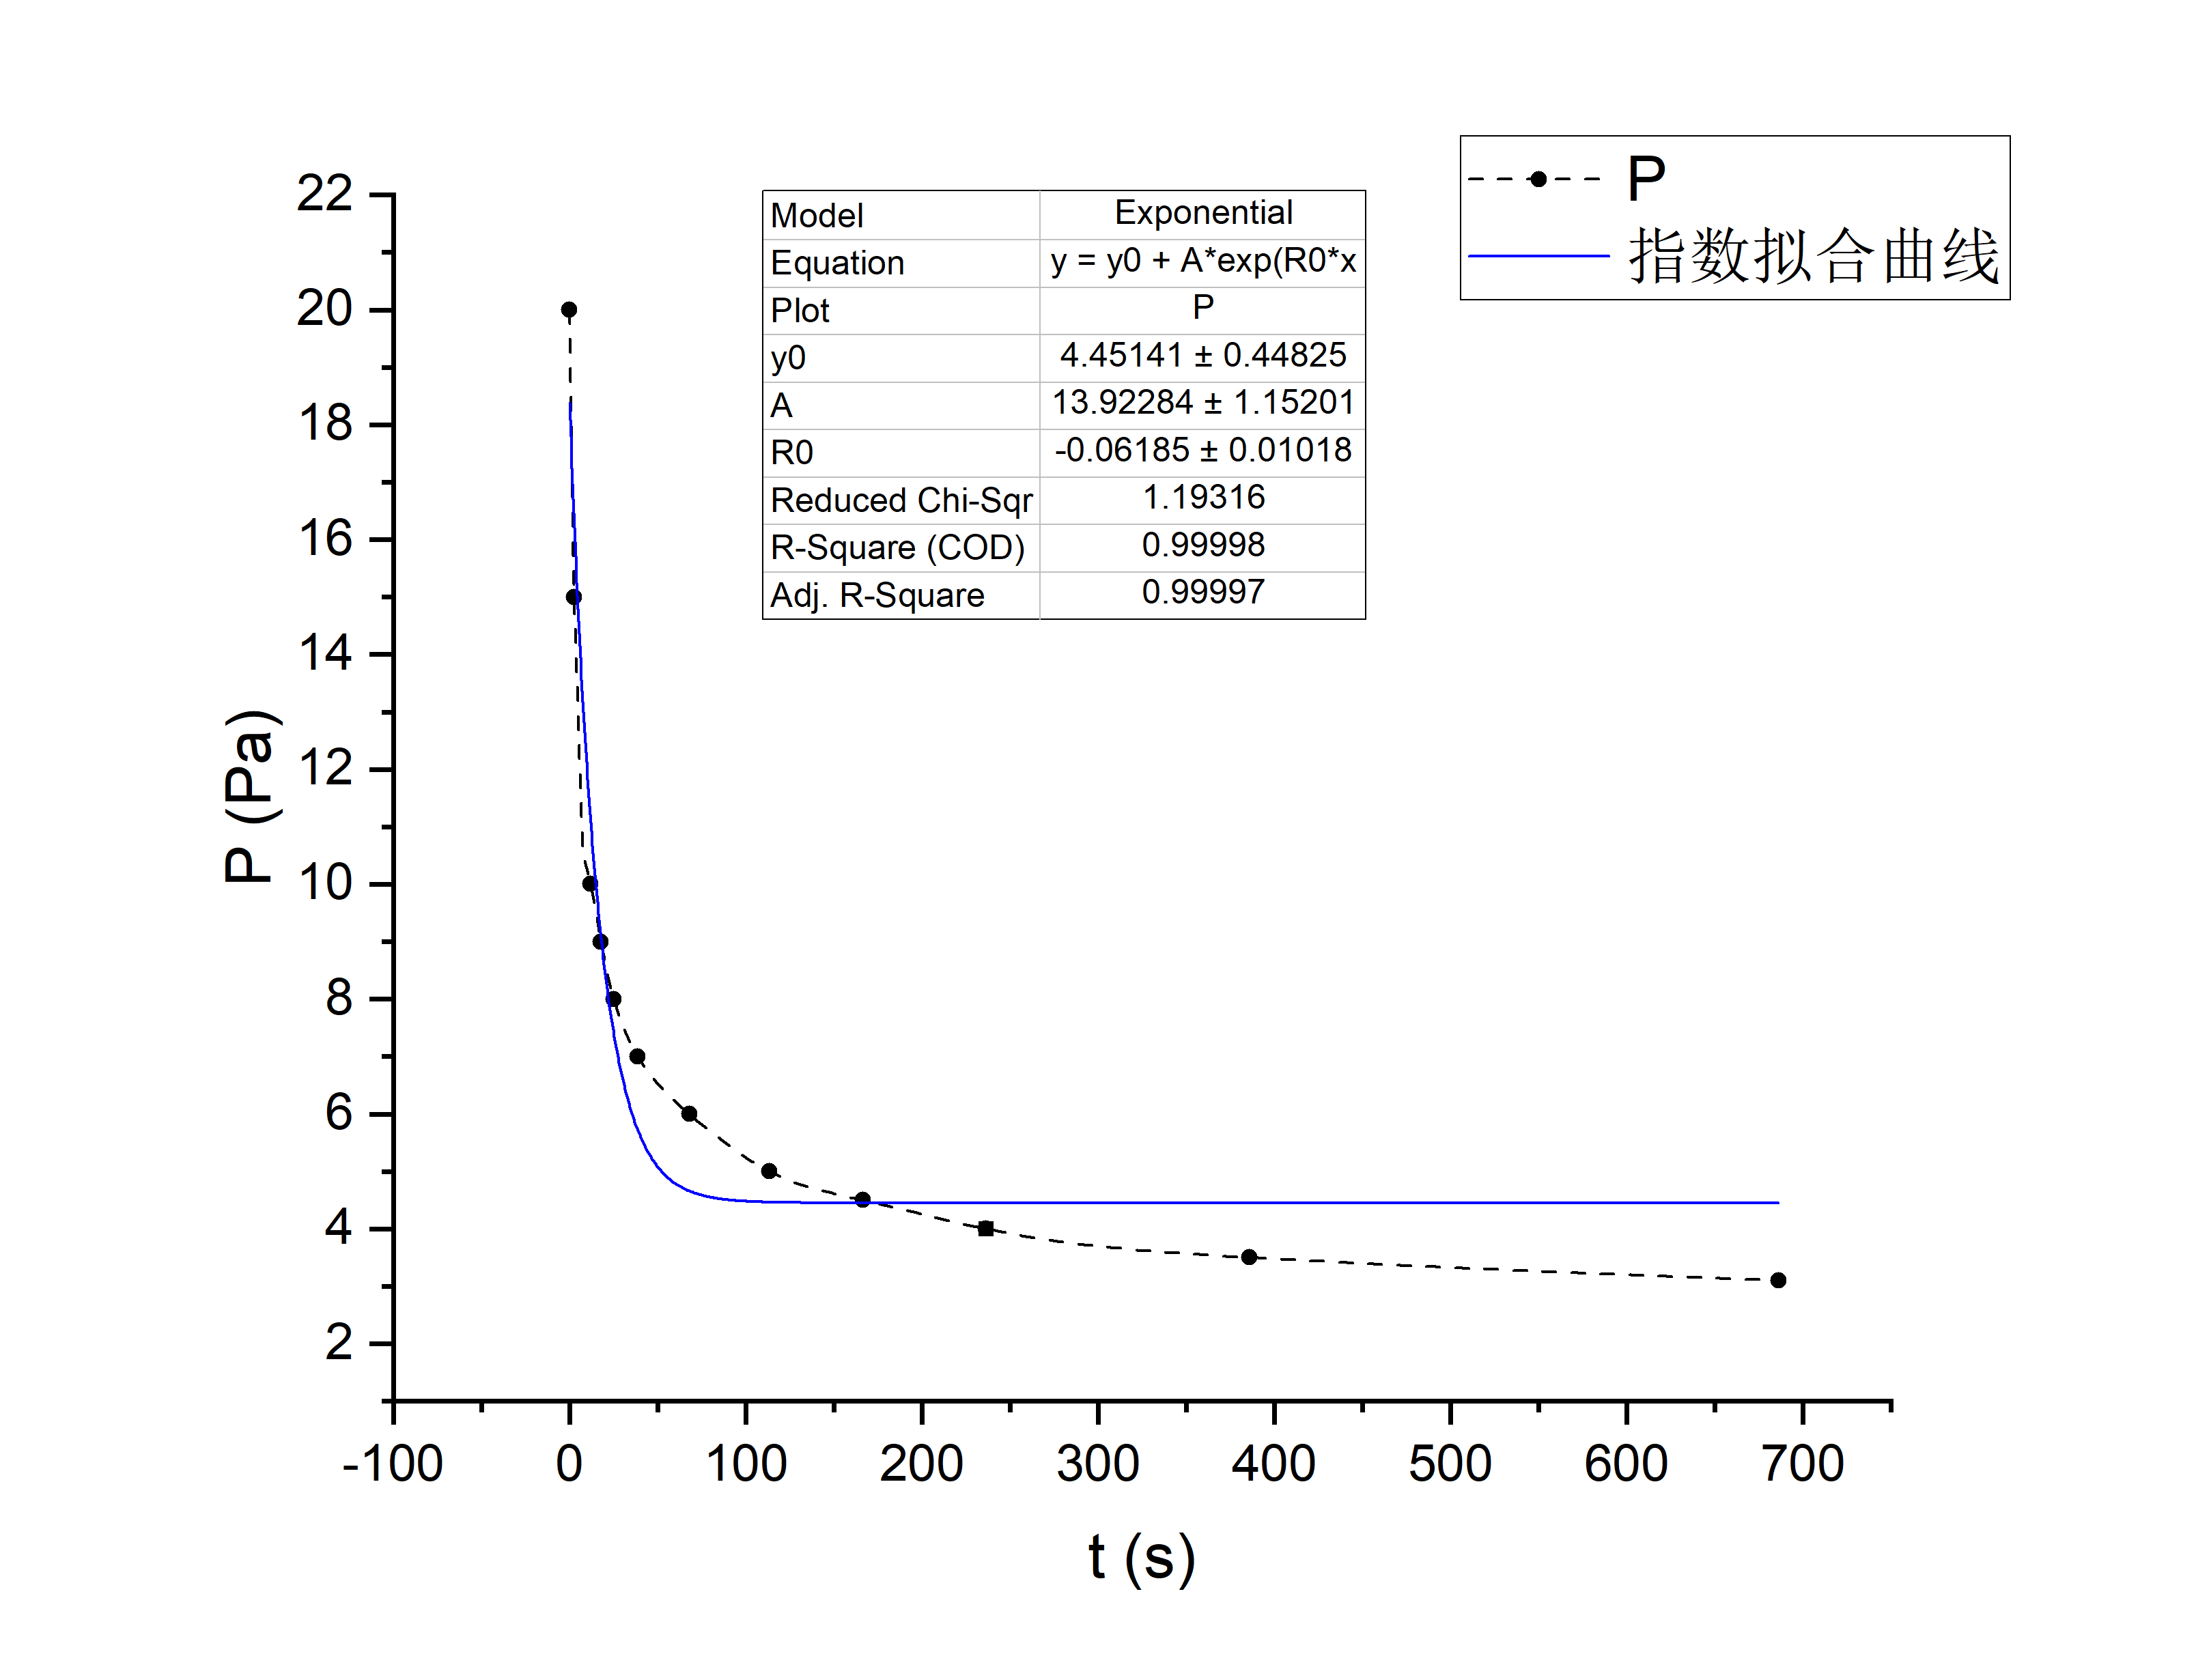
\includegraphics[scale=0.45]{Graph2.png}
	\caption{低真空下的 $P-t$ 图}
\end{figure}
\par
从图中可以看出,低真空下的压强变化整体上满足指数曲线,但是由于抽速的减小,还有测量的误差,与拟合的曲线并不十分相符。
\subsection{粗真空}
由于第二组数据更符合实验要求,我们采用第二组数据,并减去零点误差 $P_1 = 0.2 \times 10 ^ 5 \; Pa$:
\begin{table}[!htbp]
	\centering
	\begin{tabular}{|c|c|c|c|c|c|c|c|c|c|c|c|c|c|}
		\hline
		压强 $P(\times10^5\;Pa)$ & 7.8 & 7.3 & 6.8 & 6.3 & 5.8 & 5.3 & 4.8 & 4.3 & 3.8 & 3.3 & 2.8 & 2.3 & 1.8 \\
		\hline
		$\ln{P/P_0}$ & 2.05 & 1.99 & 1.92 & 1.84 & 1.76 & 1.67 & 1.57 & 1.46 & 1.34 & 1.19 & 1.03 & 0.83 & 0.59 \\
		\hline
		时间 $t(s)$ & 0.0 & 2.0 & 4.0 & 6.4 & 9.0 & 11.8 & 15.2 & 18.8 & 22.6 & 27.2 & 32.4 & 38.3 & 45.3 \\
		\hline
	\end{tabular}
\end{table}
\par
其中$P_0 = 10^5 \; Pa$。
\par
作$\ln{P} - t $图并线性拟合:
\begin{figure}[htb]
	\centering
	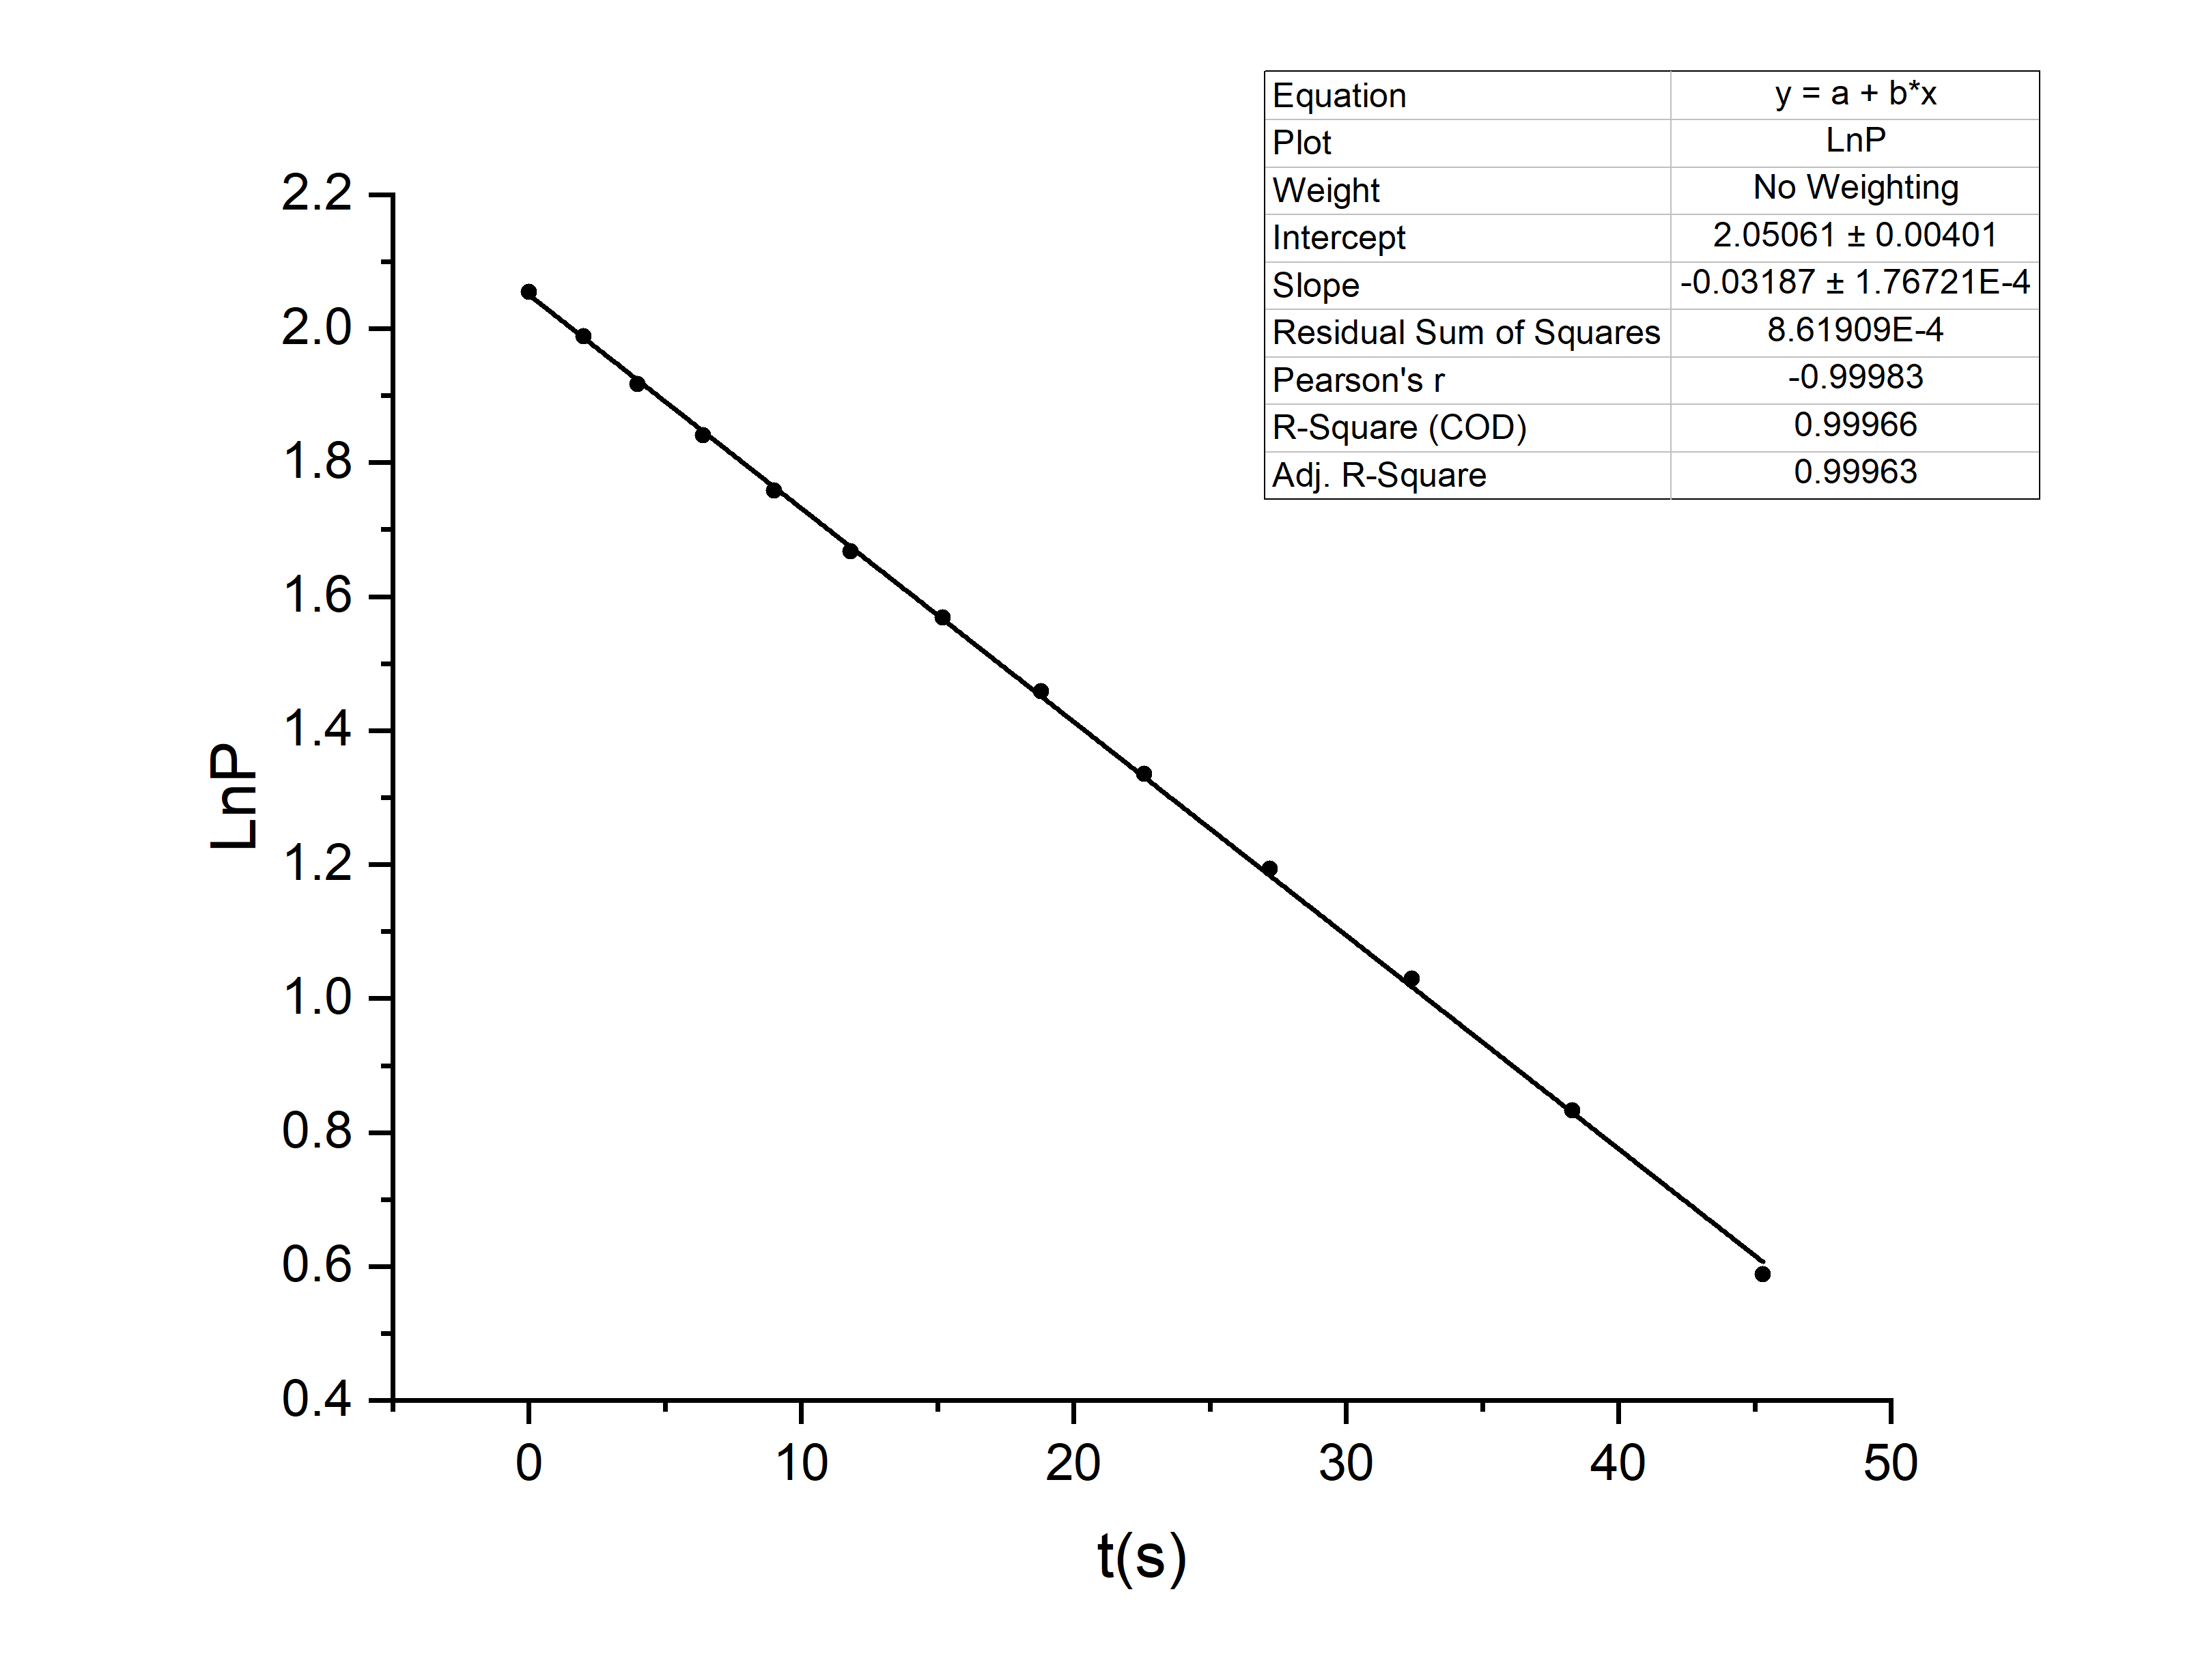
\includegraphics[scale=0.45]{Graph4.png}
	\caption{粗真空下的 $lnP-t$ 图}
\end{figure}
\par
从图中可以我们可以发现,$lnP$与时间$t$有比较好的线性关系,我们可以得到直线的斜率:
$$ k = -\frac{S}{V} = -0.032 \; s^{-1}$$
\par
代入$V = 2L $从而可以得到抽速:
$$ S = -kV = 0.064 \; L/s $$

\subsection{放电现象与真空度的关系}
\begin{table}[!htbp]
	\centering
	\begin{tabular}{|c|c|c|c|c|}
		\hline
		气压范围($Pa$) & $10^3$及以上 & $10^2$ & $10^1 $ & $10^0$ \\
		\hline
		放电颜色 & 无色 & 紫红色 & 浅红色 & 浅蓝色(玻璃荧光) \\
		\hline
	\end{tabular}
\end{table}
\par
与讲义所给的表格有部分不太符合,未观察到灰白色,该范围基本都是浅蓝(玻璃荧光)色,这可能是真空度不均匀还有灰白色不易观察造成的。

\end{document}